
\section{Frontend that we know}
\begin{frame}
  \frametitle{Frontend that we know}
Now we are going to talk about approaches used at today's systems. \newline

I use the example of the blog app:
\begin{itemize}
	\item Service which manage users, authentication etc.
	\item Service for articles (listing, creating, editing, etc.)
	\item Frontend is SPA/SPA like
\end{itemize}
\end{frame}


\subsection{Monolith}

\begin{frame}
	\frametitle{Monolith}
	It's important to understand something about structure of application.
	So, we have one big block of code:
	\begin{figure}
		\centering
		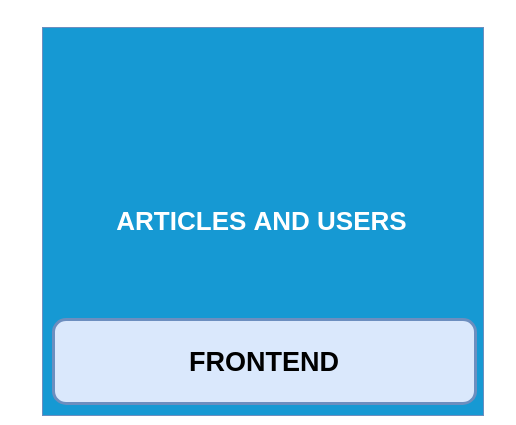
\includegraphics[width=0.6\linewidth]{pictures/monolit.png}		
		\label{fig:monolit}
	\end{figure}
\end{frame}

\begin{frame}
	\frametitle{Pros\&Cons}
	\begin{columns}[t]
		\column{0.5\linewidth}
			\textbf{\begin{center}
				+
			\end{center}}
		
		\begin{itemize}
			\item Everything at one place
			\item Probably - at one pull request we can add new feature 
			\item Deployed once with a frontend. We are sure that both layers work fine together
		\end{itemize}
		\pause
		
		\column{0.5\linewidth}
			\textbf{\begin{center}
				--
			\end{center}}
		
		\begin{itemize}
			\item Vertical scalability
			\item Complex inside
			\item A lot of legacy code can exist
			\item High entry threshold
		\end{itemize}
	
	\end{columns}
\end{frame}

\subsection{Microservices}

\begin{frame}
\frametitle{Microservices}
	\begin{figure}
		\centering
		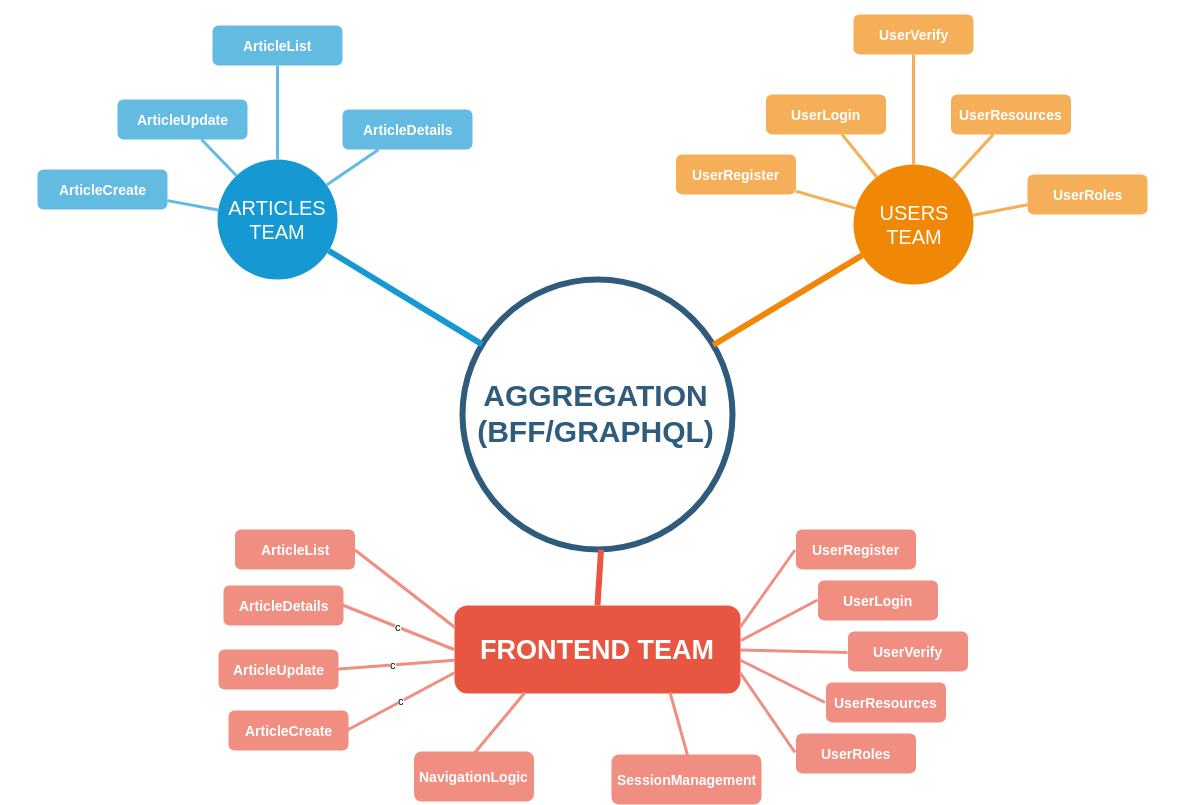
\includegraphics[width=0.8\linewidth]{pictures/microservices-knowledge.png}		
		\label{fig:microservices}
	\end{figure}
\end{frame}

\begin{frame}
\frametitle{Pros\&Cons}
\begin{columns}[t]
	\column{0.5\linewidth}
	\textbf{\begin{center}
			+
	\end{center}}
	
	\begin{itemize}
    	\item Working parallel \pause
		\item Many smaller codebases \pause
		\item This codebases are really small \pause
		\item Microservices are trendy now \pause
		\item We can use a lot of cool tools\pause
		\item We are still skipping performance and scalability
	\end{itemize}\pause
	
	
	\column{0.5\linewidth}
	\textbf{\begin{center}
			--
	\end{center}}
	
	\begin{itemize}
		\item Many codebases - additional automation costs
		\item Integration needed (+ more testing etc.)
		\item Infrastructural costs
		\item Eventual consistency
		\item ...
		\item Just a lot of work more
	\end{itemize}
	
\end{columns}
\end{frame}


